\documentclass[a4paper]{article}
\usepackage[english,spanish]{babel}  %  Tipografia, fecha y idioma de los formatos del documento
\usepackage[latin1]{inputenc}  %  Acentos
\usepackage[T1]{fontenc}  %  Acentos en el archivo .dvi
\usepackage{amsmath} % Math�matiques symbols
\usepackage{amsfonts}
\usepackage{graphicx}
\usepackage{float}
\begin{document}  %  Inicio del documento
\selectlanguage{english}  %  Seleccion del idioma
\title{Quadrotor Model}  %  titulo general del documento
\author{Colmenares V. Josu�}  %  Nombre del autor que aparecera en el titulo
\date{June 2014}  %  Fecha que aparecera en el titulo
\maketitle{}  %  Forza a Latex a escribir le titulo en esta ubicacion
\tableofcontents{}  %  Escribe la tabla de contenido (el indice).
\newpage
\section{Basis Concepts}  %  Titulo del parrafo Titre  de  paragraphe
\subsection{Inertia Moments}
The inertia moment of a body represents a \emph{resistance} to change its velocity of rotation. If a body has masse, so it has also a moment of inertia relative to some axe. Let us determine the inertia moment $J_{e}$ around the axis $\bf{e}$ as shown in the next figure:
\begin{center}
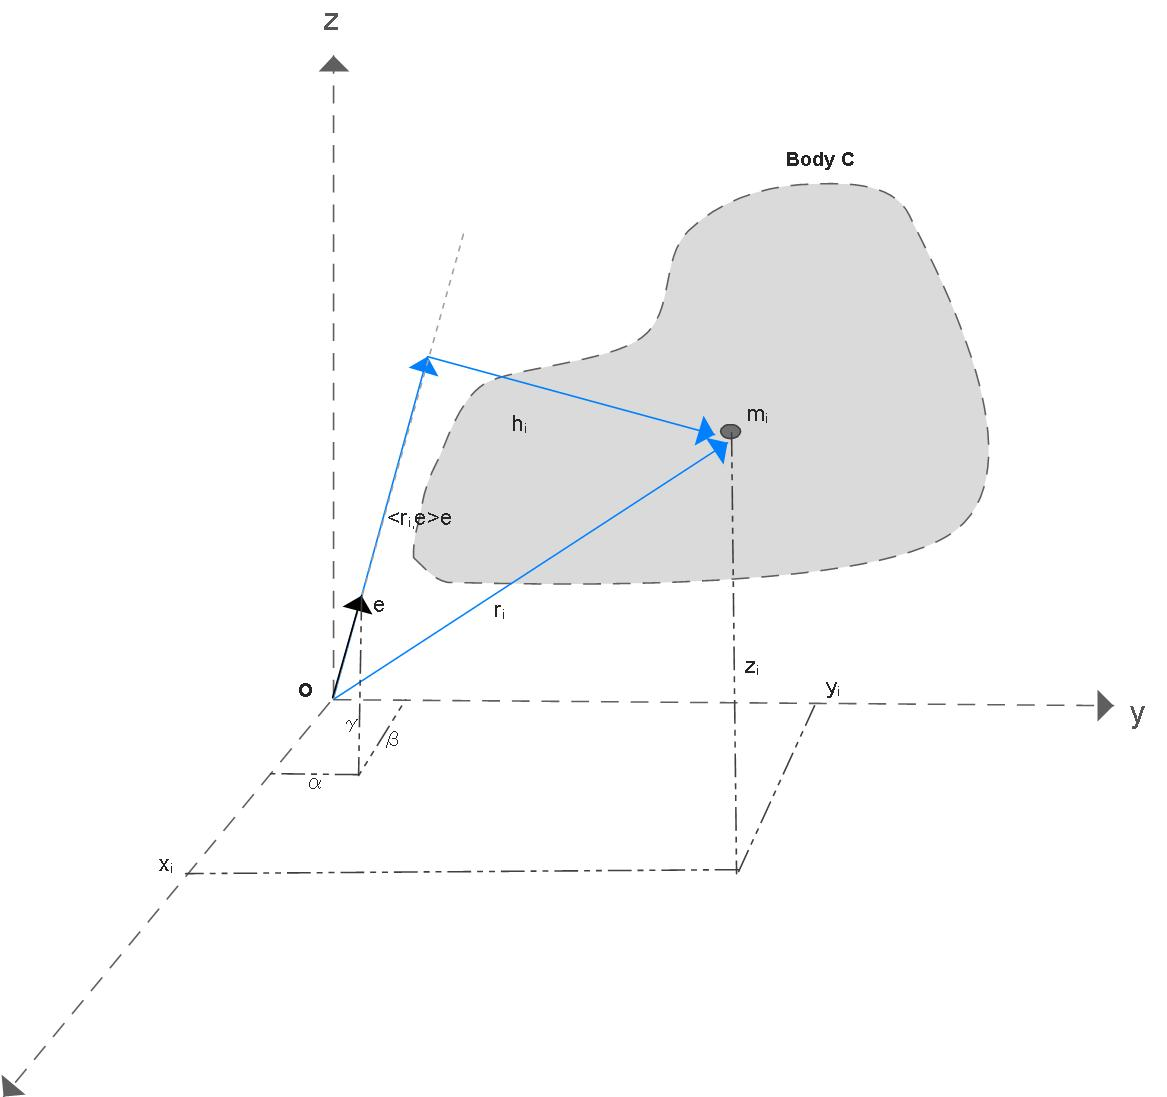
\includegraphics[scale=0.25]{Inertia_moments}
\end{center}
\[ J_{e}=\sum_{i \in C} m_{i}{h_{i}}^{2}\]
where
\[{h_{i}}^{2}=<r_{i},r_{i}>-<r_{i},e> \]
With $<*,*>$ as the inner product and
\[ r_{i}=(x_{i},y_{i},z_{i})^{T}\]
\[ e=(\alpha,\beta,\gamma)^{T} \qquad \|e\|=1 \]
Therefore,
\[ {h_{i}}^{2} = {x_{i}}^{2}+{y_{i}}^{2}+{z_{i}}^{2}-\alpha^{2}{x_{i}}^{2}-\beta^{2}{y_{i}}^{2}-\gamma^{2}{x_{i}}^{2} -2 \alpha \beta x_{i} y_{i} -2\beta\gamma y_{i} z_{i} -2\alpha \gamma x_{i} z_{i}  \]
and provided
\[ \alpha^{2}+\beta^{2}+\gamma^{2}=1 \]
\[ {h_{i}}^{2} = \alpha^{2}({y_{i}}^{2}+{z_{i}}^{2})+\beta^{2}({x_{i}}^{2}+{z_{i}}^{2})+\gamma^{2}({{x_{i}}^{2}+y_{i}}^{2})-2 \alpha \beta x_{i} y_{i} -2\beta\gamma y_{i} z_{i} -2\alpha \gamma x_{i} z_{i}  \]
Consequently,
\[ \begin{array}{rcl} 
J_{e} & = &\displaystyle {\alpha^{2} \sum_{i \in C} m_{i}({y_{i}}^{2}+{z_{i}}^{2}) + \beta^{2}\sum_{i \in C} m_{i}({x_{i}}^{2}+{z_{i}}^{2}) + \gamma^{2} \sum_{i \in C} m_{i}({{x_{i}}^{2}+y_{i}}^{2})} \\
\mbox{} &  &\displaystyle { -2 \alpha \beta \sum_{i \in C} m_{i}x_{i} y_{i} -2\beta\gamma  \sum_{i \in C} m_{i}y_{i} z_{i} -2\alpha \gamma  \sum_{i \in C} m_{i}x_{i} z_{i}}  \end{array} \]
The following expressions are called \emph{main inertia moments}:
\[J_{xx}:=\sum_{i \in C} m_{i}({y_{i}}^{2}+{z_{i}}^{2})\quad J_{yy}:=\sum_{i \in C} m_{i}({x_{i}}^{2}+{z_{i}}^{2}) \quad J_{zz}:=\sum_{i \in C} m_{i}({{x_{i}}^{2}+y_{i}}^{2}) \]
And the quantities:
\[J_{xy}:=\sum_{i \in C} m_{i}x_{i} y_{i} \quad J_{xz}:=\sum_{i \in C} m_{i}x_{i} z_{i} \quad J_{yz}:=\sum_{i \in C} m_{i}y_{i} z_{i} \]
They are named \emph{centrifugal inertia moments}. By consequence, the inertia moment can be rewritten as: 
\[ J_{e}=<e,\mathbb{J}e> \]
With
\[ \mathbb{J}=\left( \begin{array}{ccc}
J_{xx} & -J_{xy} & -J_{xz} \\
-J_{yx}& J_{yy} & -J_{yz} \\
-J_{zx}& -J_{zy} & J_{zz}
\end{array} \right) \]
\[ J_{xy}=J_{yx} \quad J_{xz}=J_{zx} \quad J_{yz}=J_{zy} \]
$\mathbb{J}$ is named the \emph{inertia tensor}. This inertia tensor is useful to calculate the kinectic energy $T_{rel,O}$ and the impulse moment $K_{rel,O}$ of a body rotating around a pivot $O$:
\[ K_{rel,O}=\mathbb{J}w \qquad T_{rel,O}=\frac{1}{2}w^{T}\mathbb{J}w \] 
Where $w$ is the angular velocity of the body.
\subsection{Skew symmetric Matrix}
 The following vectorial product:
\[ c=[a,b] \]
can be represented as a product between a matrix and a vector:
\[ c= Ab \]
where $A$ will be obtained from the vector $a$. For instance:
\[ a=\left( \begin{array}{c}
 a_{1} \\ a_{2} \\ a_{3} \end{array}
 \right) \Longrightarrow
A=
\left(
\begin{array}{ccc}
0 & -a_{3} & a_{2} \\ a_{3} & 0 & -a_{1} \\ -a_{2} & a_{1} & 0
\end{array} 
\right)
\]
Consequently, the vectorial product with the angular velocity $[\omega,\cdot]$ can be expressed by a matrix $W$:
\[ W= \left( \begin{array}{ccc} 
0 & -w_{3} & w_{2} \\ w_{3}&0&-w_{1} \\ -w_{2}& w_{1} &0
\end{array} \right)
\] 
This matrix is named the \emph{skew symmetric matrix}.
\subsection{Change of coordinates}
Let be two coordinated systems $S_{1}$ and $S_{2}$ and a matrix $T$ such that any vector $r$ whose coordinates are expressed in $S_{2}$ can be expressed in $S_{1}$ as:
\[ \underset{S_{1}}{r}=T \underset{S_{2}}{r} \]
The matrix $T$ is a transformation matrix. The coordinated systems will be defined by their vectorial basis:
\[ S_{1}=(i_{1},j_{1},k_{1})\qquad S_{2}=(i_{2},j_{2},k_{2})\]
Let's suppose it is known the coordinates of each basis vector of system $S_{2}$ and thus the transformation matrix can be written as:
\[ T=\left( 
\begin{array}{ccc}
<i_{2},i_{1}> & <j_{2},i_{1}> & <k_{2},i_{1}> \\
<i_{2},j_{1}> & <j_{2},j_{1}> & <k_{2},j_{1}>\\
<i_{2},k_{1}> & <j_{2},k_{1}> & <k_{2},k_{1}>\\
\end{array}
\right) \]
Where $<*,*>$ is the inner product and it defines the projection of one vector over another.
\subsection{Rotation Matrix}
A rotation matrix is a matrix $R \ \in \ \Re^{3x3}$ such that:
\[ |Rr|=|r| \]
A rotation matrix satifies the following properties:
\begin{itemize}
\item[\bf{P1}] $R^{T}=R^{-1}$
\item[\bf{P2}] $|\rm{det}(R)|=1$
\item[\bf{P3}] The eigenvectors and eigenvalues of $R$ are: 
\[ 
\begin{array}{rcl}
\lambda_{1}&=&1\\
\lambda_{2}&=&\cos(\theta)+i\sin(\theta)\\
\lambda_{2}&=&\cos(\theta)-i\sin(\theta)
\end{array}
\]
With $\displaystyle \cos(\theta)=\frac{{\rm Tr}(R)-1}{2}$
\end{itemize}
Let us suppose it is known the new basis vectors obtained after the application of a rotation, that is:
\[S_{2}=(i^{'},j^{'},k^{'}) \]
Where:
\[ 
\begin{array}{rcl}
i^{'}&=&Ri\\
j^{'}&=&Rj\\
k^{'}&=&Rk
\end{array}
\]
Therefore, the matrix rotation $R$ can be expressed as:
\[ R=\left( 
\begin{array}{ccc}
<i^{'},i> & <j^{'},i> & <k^{'},i> \\
<i^{'},j> & <j^{'},j> & <k^{'},j>\\
<i^{'},k> & <j^{'},k> & <k^{'},k>\\
\end{array}
\right) \]
\subsubsection{Rotations about axes x, y and z}
Let us have a rotation about the axis $x$ like it is shown in the next figure:
\begin{center}
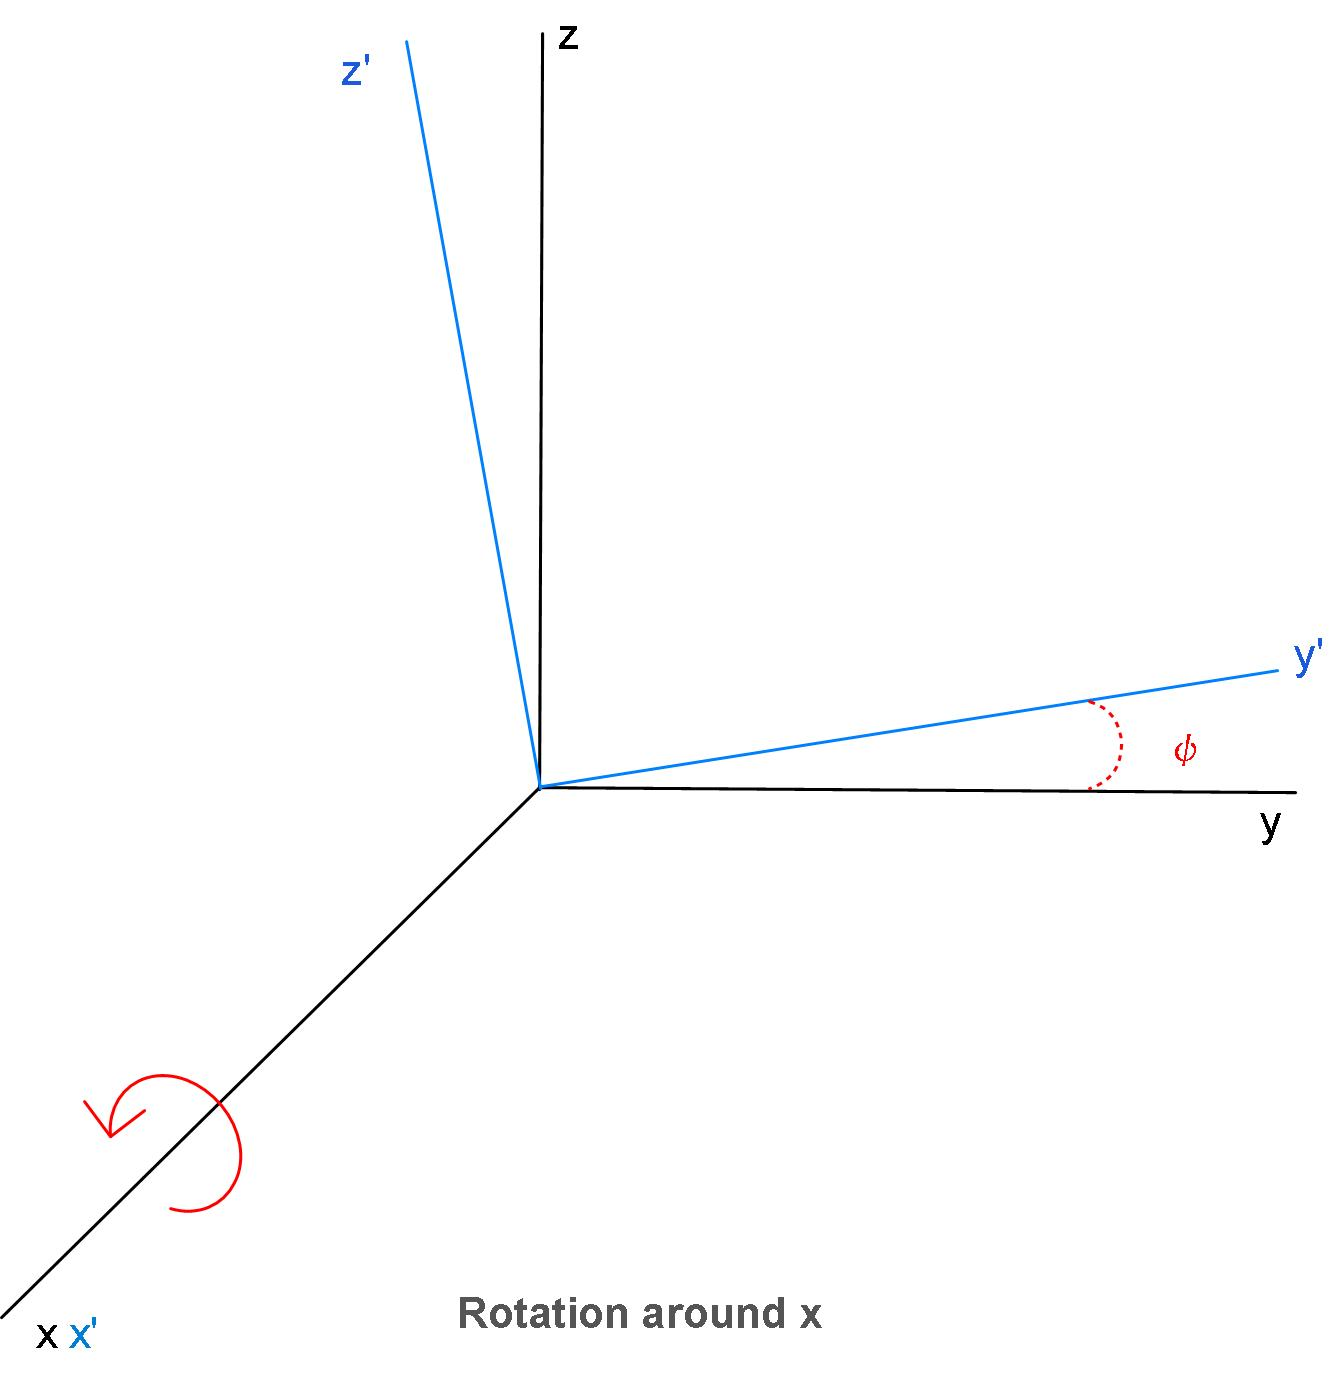
\includegraphics[scale=0.15]{Rotation_x}
\end{center}
Then, applying the expression for $R$, it yields:
\[ 
R_{x}=\left( 
\begin{array}{ccc}
1&0&0\\
0&\cos(\psi)&-\sin(\psi)\\
0&\sin(\psi)&\cos(\psi)
\end{array}
\right)
\]
In a similar way, the rotations about $y$ and $z$ 
\begin{center}
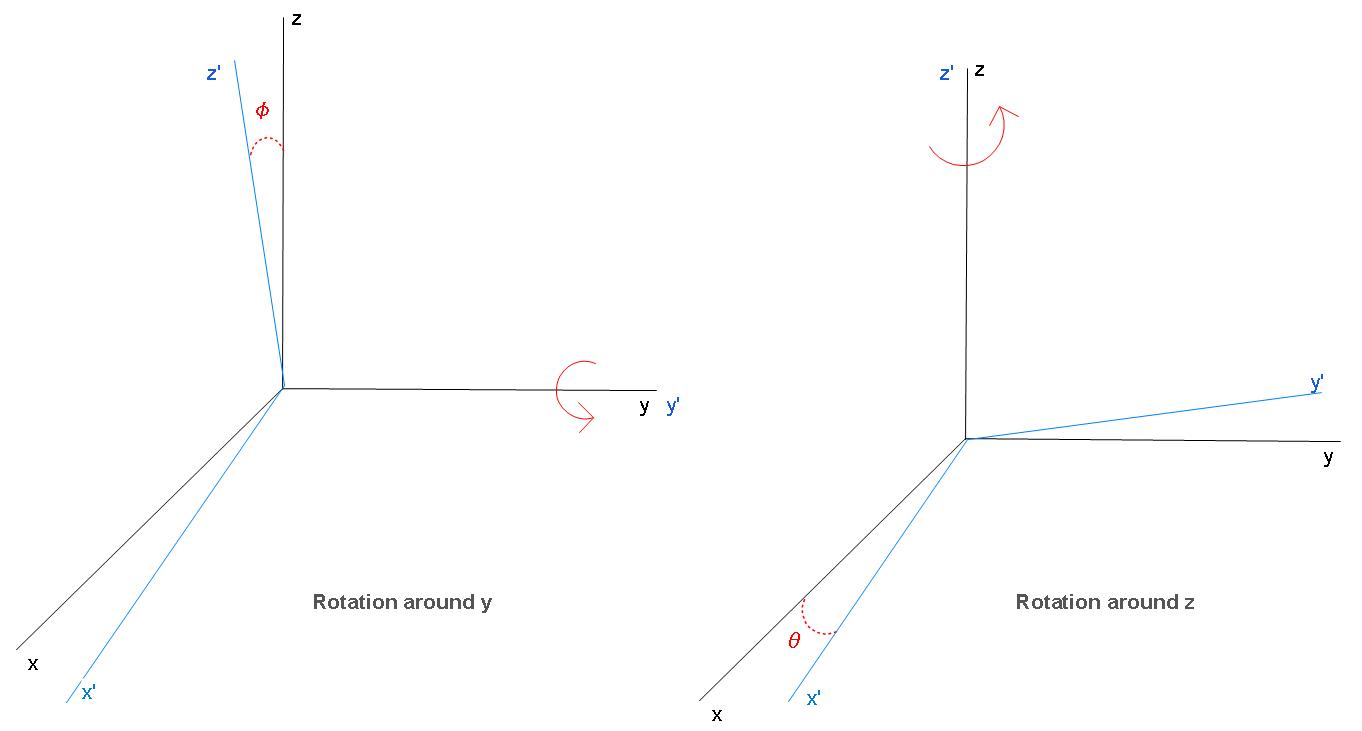
\includegraphics[scale=0.25]{Rotations_y_z}
\end{center}
They yield:
\[ 
R_{y}=\left( 
\begin{array}{ccc}
\cos(\phi)&0&\sin(\phi)\\
0&1&0\\
-\sin(\phi)&0&\cos(\phi)
\end{array}
\right)
\mbox{}
R_{z}=\left( 
\begin{array}{ccc}
\cos(\theta)&-\sin(\theta)&0\\
\sin(\theta)&\sin(\theta)&0\\
0&0&1
\end{array}
\right)
\]
\subsubsection{Composition of rotations}
Let us have two rotation matrices $R_{1}$ and $R_{2}$, so it is possible to replace this two matrix by only one rotation matrix $R$.
\paragraph{Rotations in the same coordinated system}
In this case, second rotation is applied after the first one but relative to the same frame,
\begin{center}
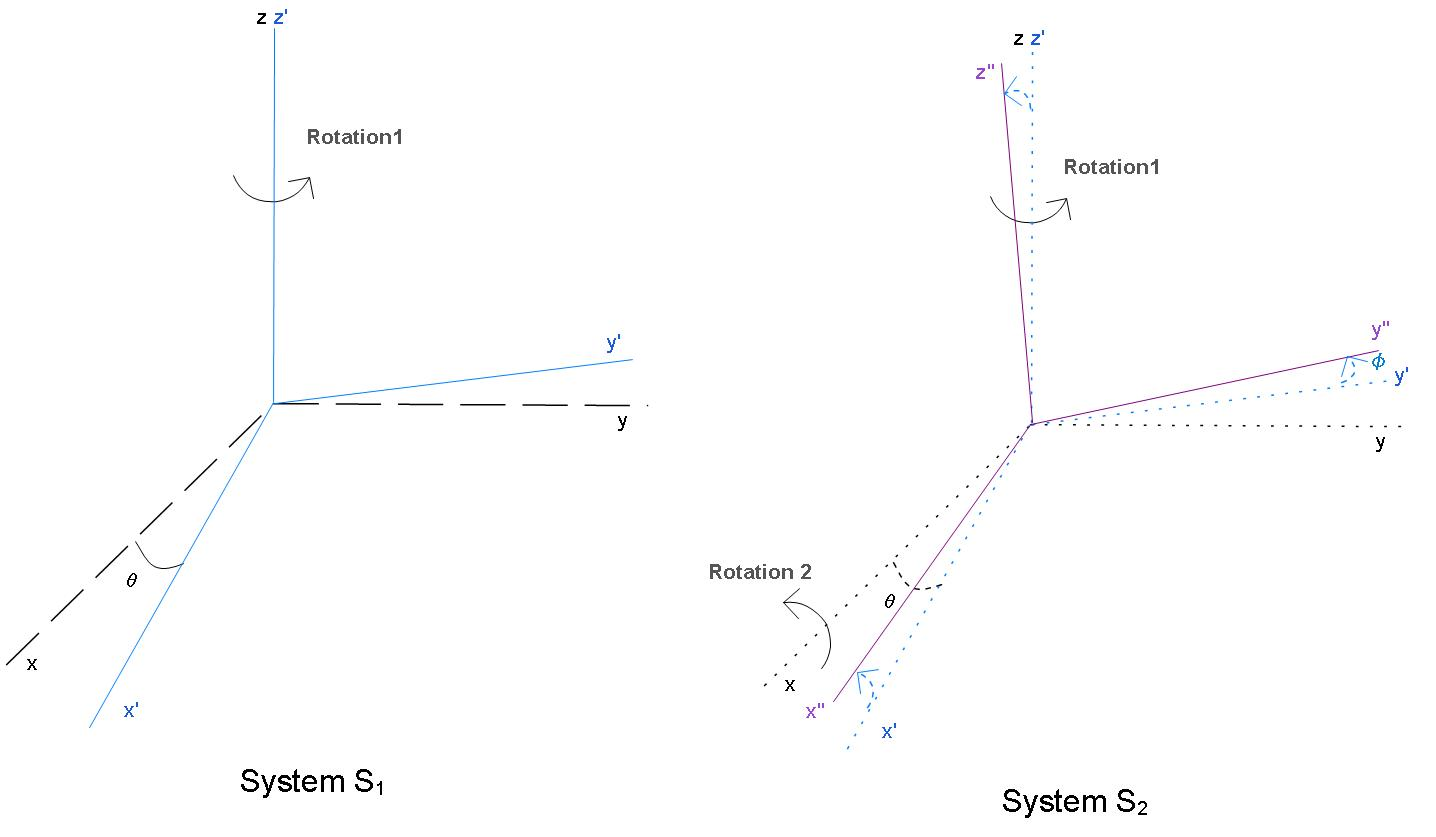
\includegraphics[scale=0.23]{Rotation_same_axis}
\end{center}
Thus, it results:
\[ r^{''}=R_{2}r^{'}=R_{2}(R_{1}r)\]
Or
\[ r^{''}=Rr\]
With $R=R_{2}R_{1}$
\paragraph{Rotations in different coordinated systems}
In this case, there are two rotation matrices $R_{1}$ and $R_{2}$ defined in the basis $S$ and $S_{1}$ respectively. $R_{1}$ will be applied first to the vector $r$ in $S$ and after it will be applied $R_{2}$ to the vector $r^{'}$ in $S_{1}$
\[ S \overset{R_{1}}{\longrightarrow} S_{1} \overset{R_{2}}{\longrightarrow} S_{2}\]
\begin{center}
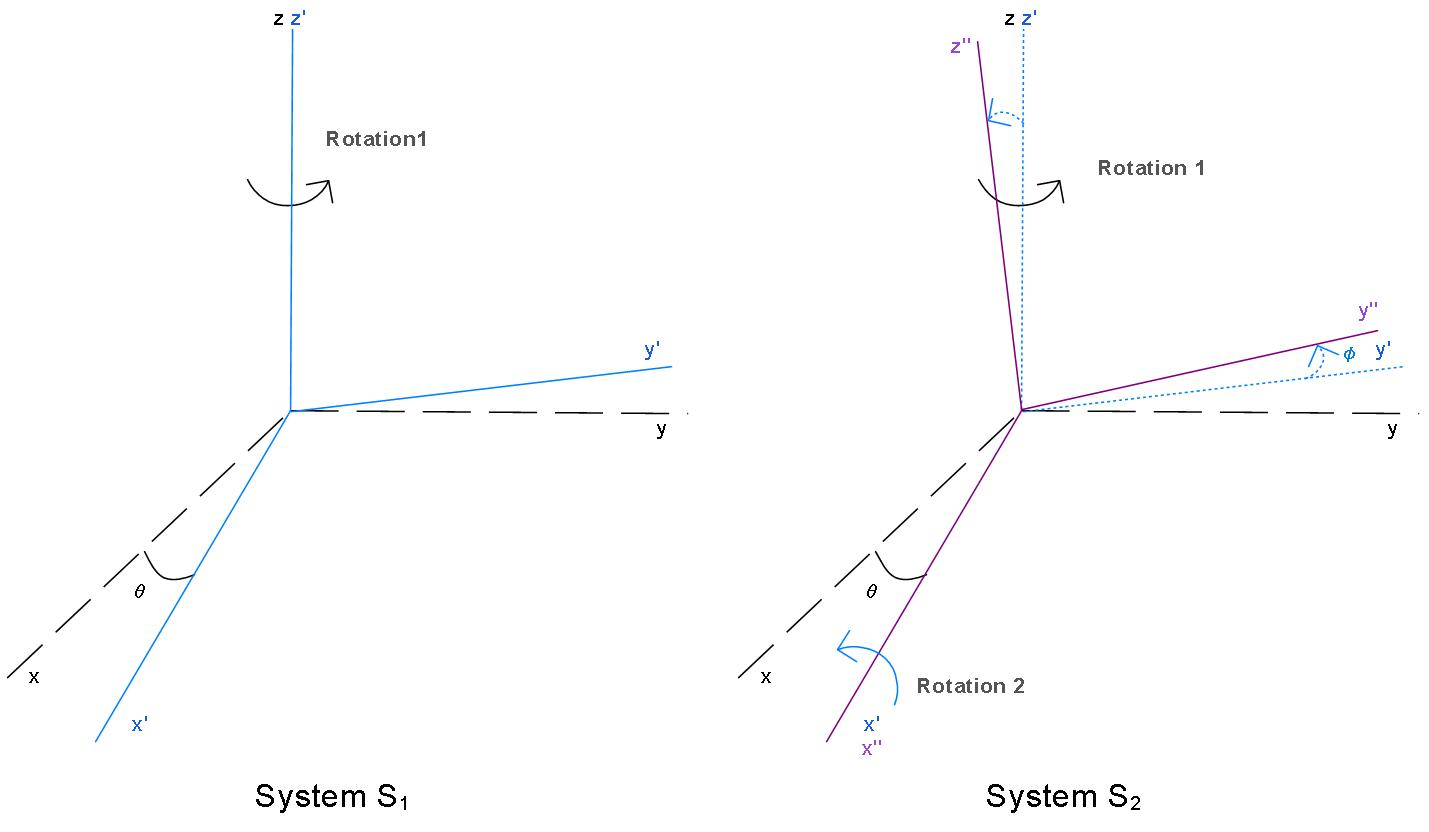
\includegraphics[scale=0.23]{Rotation_different_axes}
\end{center}
The rotation matrix resulting will be:
\[ R=R_{1}R_{2} \qquad {\rm such \ that} \qquad \underset{S}{r^{''}}=R \underset{S}{r}\]
In other words, when the second rotation is carried out in the new basis vectors $(i^{'},j^{'},k^{'})$, the resulting rotation is obtained from a post-multiplication. In the other side, when the rotations are in the same coordinated system, the resulting rotation is obtained from a pre-multiplication.
\subsubsection{Transformation of coordinates caused by a rotation matrix}
A rotation matrix generates a new coordinated system due to rotation of a set of basis vectors $(i,j,k)$ as it is shown in the next figure:
\[ S \overset{R_{1}}{\longrightarrow} S_{1} \]
\begin{center}
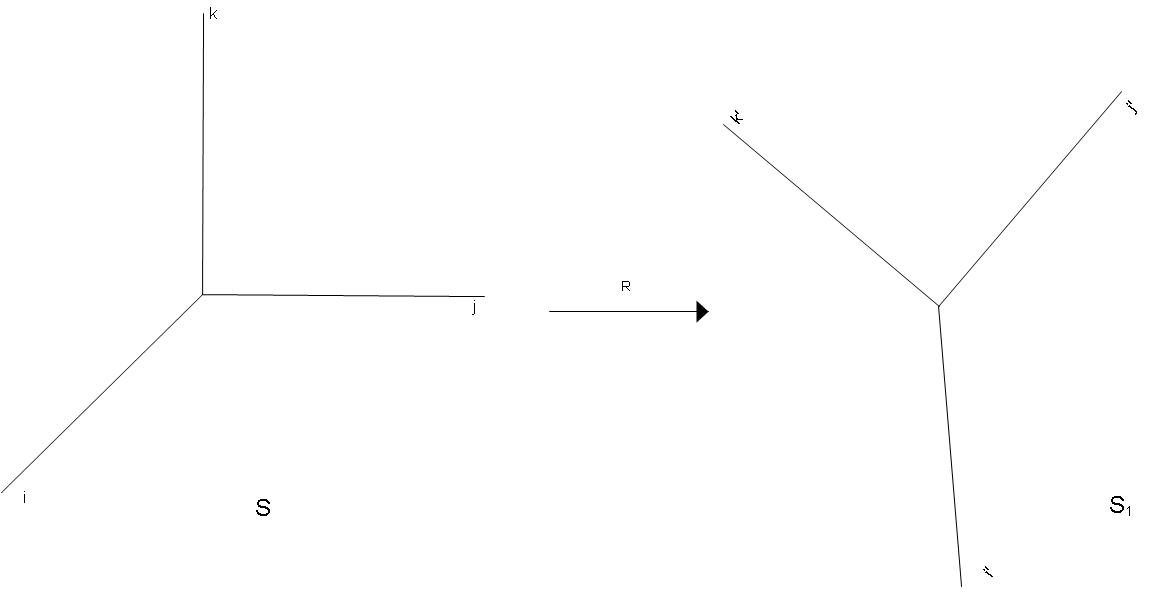
\includegraphics[width=10cm,height=5.5cm]{Rotated_System}
\end{center}
The new basis vectors result from the rotation of the original basis vectors:
\[ (i^{'},j^{'},k^{'})=R(i,j,k) \]
Any vector $\bf r$ expressed in system $S_{1}$ can be expressed in the system $S$ by doing:
\[ 
\left( \begin{array}{c}
coords \ of\\
\rm r\\
in \ S
\end{array} \right)=R\left( 
\begin{array}{c}
coords \ of\\
\rm r\\
in \ S_{1}
\end{array}  \right)
 \]
 \subsection{Euler Angles}
The euler angles are the angles of three rotations about the axes $x$, $y$ or $z$. There are several ways to chose the rotations, for example, $(x-y'-x)''$,$(z-x'-z'')$, $(x-y'-z'')$ and so on. Here it will be chosen the rotation $(z-y'-x'')$. The angles of this rotation about three different axes is called \emph{Cardan angles} or \emph{Tait-Bryan angles}.
\subsubsection{Cardan Angles}
The rotation around the axis $z$ is named \emph{yaw}, the rotation around $y$ is named \emph{pitch} and the rotation about $x$ is named \emph{roll}. The following figures describes these three rotations:
\begin{center}
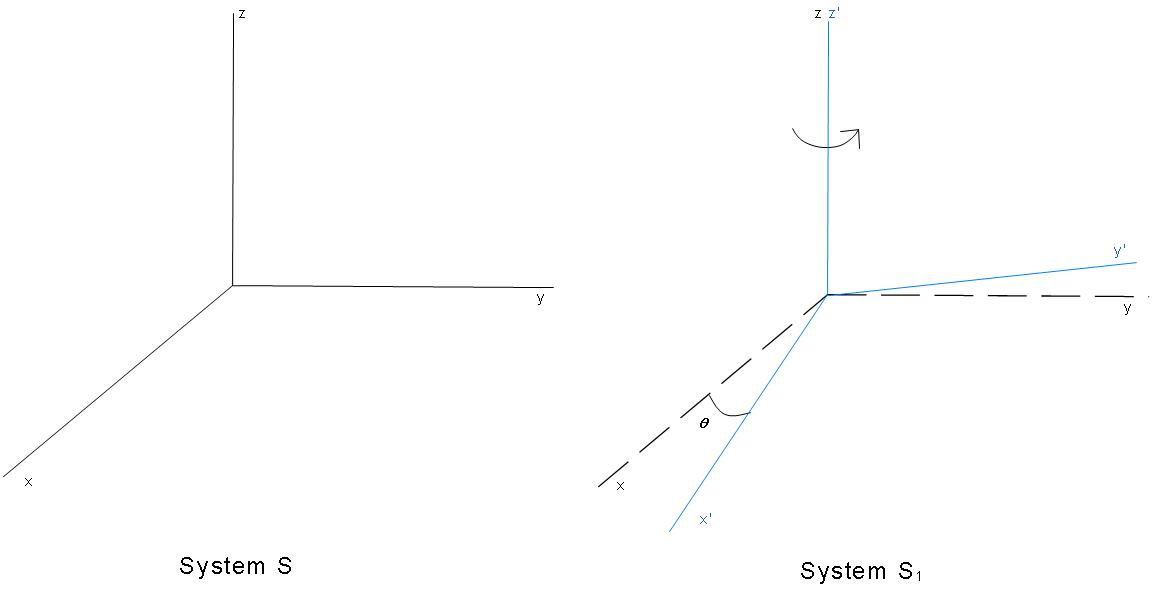
\includegraphics[scale=0.25]{S_S1}
\end{center}
\begin{center}
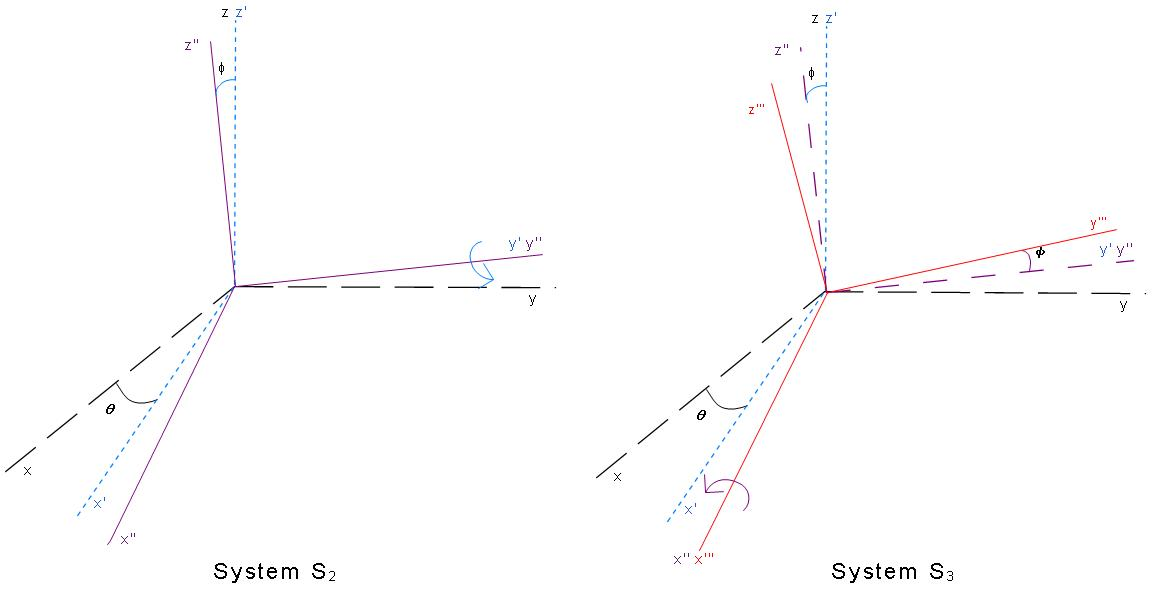
\includegraphics[scale=0.25]{S1_S2}
\end{center}
The first rotation is performed around axis $z$ and it originates the system $S_{1}$. The second rotation is done around axis $y'$ and it originates the system $S_{2}$. Finally, The third one is carried out around axis $x''$ and it originates the system $S_{3}$. The resulting rotation is given by:
\[ 
R=\left( \begin{array}{ccc}
c\theta c\phi & -s\theta c\psi+c\theta s\phi s\psi & s\theta s\psi+c\theta s\phi c\psi\\
s\theta c\phi & c\theta c\psi+s\theta s\phi s\psi & -c\theta s\psi+s\theta s\phi c\psi\\
-s\phi & c\phi s\psi & c\phi c\psi
\end{array}
\right)
\] 
Where $s\cdot$ and $c\cdot$ mean $\cos(\cdot)$ and $\sin(\cdot)$ respectively. In addition, any vector expressed in the last frame $S_{3}$ can be expressed in the first frame $S$ by means of this expresion of $R$.
\subsection{Derivative of a rotation matrix}
The derivative of a rotation is needed to know the evolution of the rotation at every time. The variation in the rotation matrix can be represented as a product of two rotations, that is:
\[ R(t+\delta t)=R(t)R(\delta t) \]
Where $R(\delta t)$ represents a rotation around the new frame determined by the matrix rotation $R(t)$. Besides, the definition of velocity and the euler theorem allow to find a relationship with the skew symmetric matrix. 
\[ v=\underset{\delta t \rightarrow 0}{\lim} \frac{r(t+\delta t)-r(t)}{\delta t}=[w,r]=Wr \]
If $r(t+\delta t)$ is a consequence of a rotation, it can be written as:
\[ r(t+\delta t)=R(\delta t)r(t) \]
Next, applying this to precedent equation:
\[ \underset{\delta t \rightarrow 0}{\lim} \frac{R(\delta t)r(t)-r(t)}{\delta t}= 
\underset{\delta t \rightarrow 0}{\lim} \frac{(R(\delta t)-I)r(t)}{\delta t} \]
\[ v= \left( \underset{\delta t \rightarrow 0}{\lim} \frac{R(\delta t)-I}{\delta t} \right)r(t) \]
Consequently,
\[ \underset{\delta t \rightarrow 0}{\lim} \frac{R(\delta t)-I}{\delta t}=W \qquad \forall r\neq 0  \]
Using the derivative's definition of a rotation matrix, it yields:
\[ \dot{R}=\underset{\delta t \rightarrow 0}{\lim}\frac{R(t+\delta t)-R(t)}{\delta t}\]
\[ \dot{R}=\underset{\delta t \rightarrow 0}{\lim}\frac{R(t)R(\delta t)-R(t)}{\delta t}= \underset{\delta t \rightarrow 0}{\lim}\frac{R(t)(R(\delta t)-I)}{\delta t}
\]
\[\dot{R}=R(t)\underset{\delta t \rightarrow 0}{\lim}\frac{R(\delta t)-I}{\delta t}=R(t)W 
\]
Finally,
\[ \dot{R}=RW \]
Where W is the skew symmetric matrix of $w$ expressed in frame generated by $R(t)$.
\subsection{Derivative of a vector expressed in a rotating frame}
Let us have two coordinated systems, the second one generated from a rotation of the first one. 
\[ S \overset{R}{\longrightarrow} S_{R} \]
In order to know the time derivative relative to system $S$ of a vector $r$ with coordinates in the system $S_{R}$, it is necessary to express that vector in coordinates relative to $S$.
\[ \frac{d}{dt}\left( \underset{\scriptscriptstyle S}{r}\right)=\frac{d}{dt}\left( Rr \right)=\frac{dR}{dt}r+R\frac{dr}{dt}=RWr+R\frac{dr}{dt} \] 
\[\frac{d}{dt}\left(\underset{\scriptscriptstyle S}{r}\right)=R\left( Wr+\frac{dr}{dt}\right) \]
\subsection{Lift and drag torque}
The airflow striking the helices generates two forces, one called \emph{lift} and another called \emph{drag}. The airflow around the helices is shown in the next figure:
\begin{center}
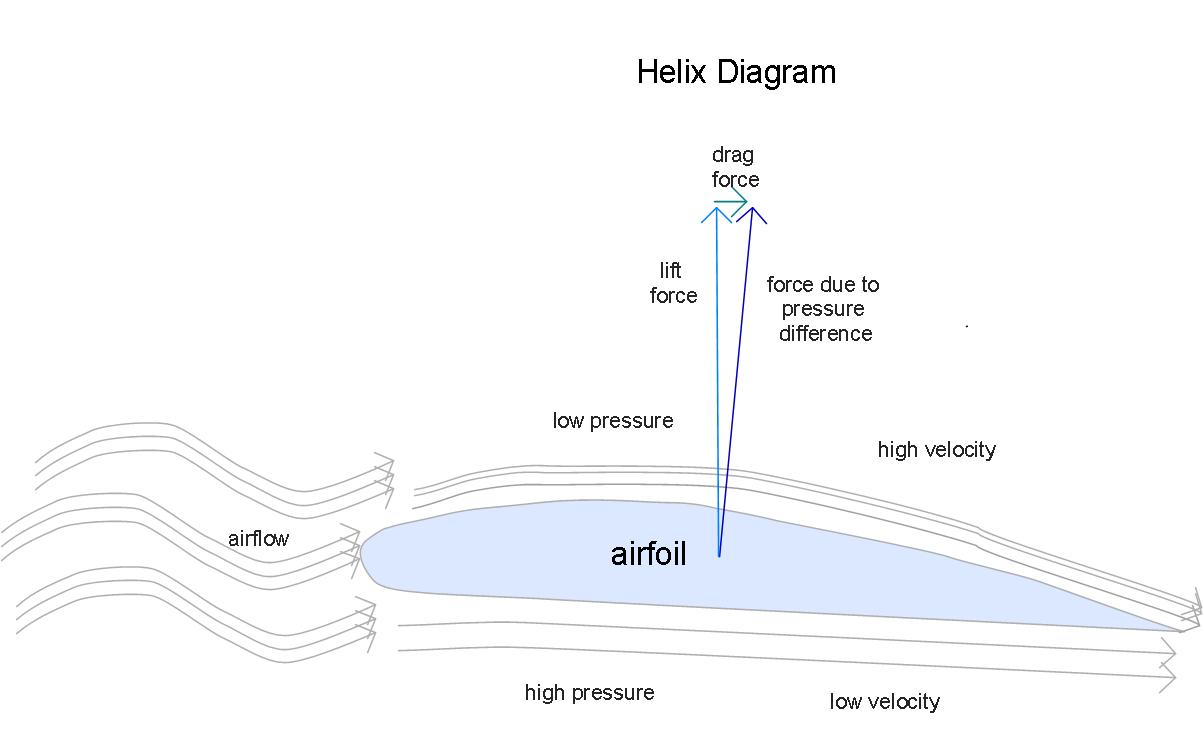
\includegraphics[scale=0.28]{Helix_diagram}
\end{center}
The low pressure is due to a high velocity and the high pressure is due to low velocity of airflow. This difference generates a force perpedicular to flow. The flow undergoes a change in direction called \emph{upward} and this change causes the apparition of drag and lift forces, as shown in next figure:
\begin{center}
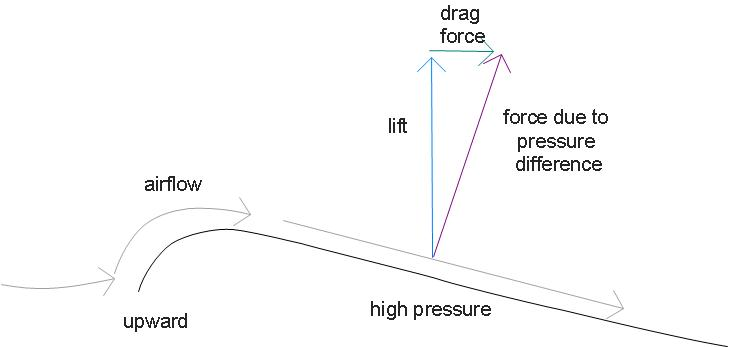
\includegraphics[scale=0.35]{Upward_flow}
\end{center}
The lift and drag forces  can be assumed to be proportional to square of velocity of helices. Thus,
\[ f_{lift}=k_{lift} w^{2}\]
\[ f_{drag}=k_{drag} w^{2}\] 
\newpage
\section{Mathematical model of a quadrotor }
The mathematical model of a quadrotor can be analyzed in two parts. One  part relative to translation and another relative to rotation.
\subsection{Position model of a quadrotor}
The nex figure describes a symmetric quadrotor with forces acting over it.
\begin{center}
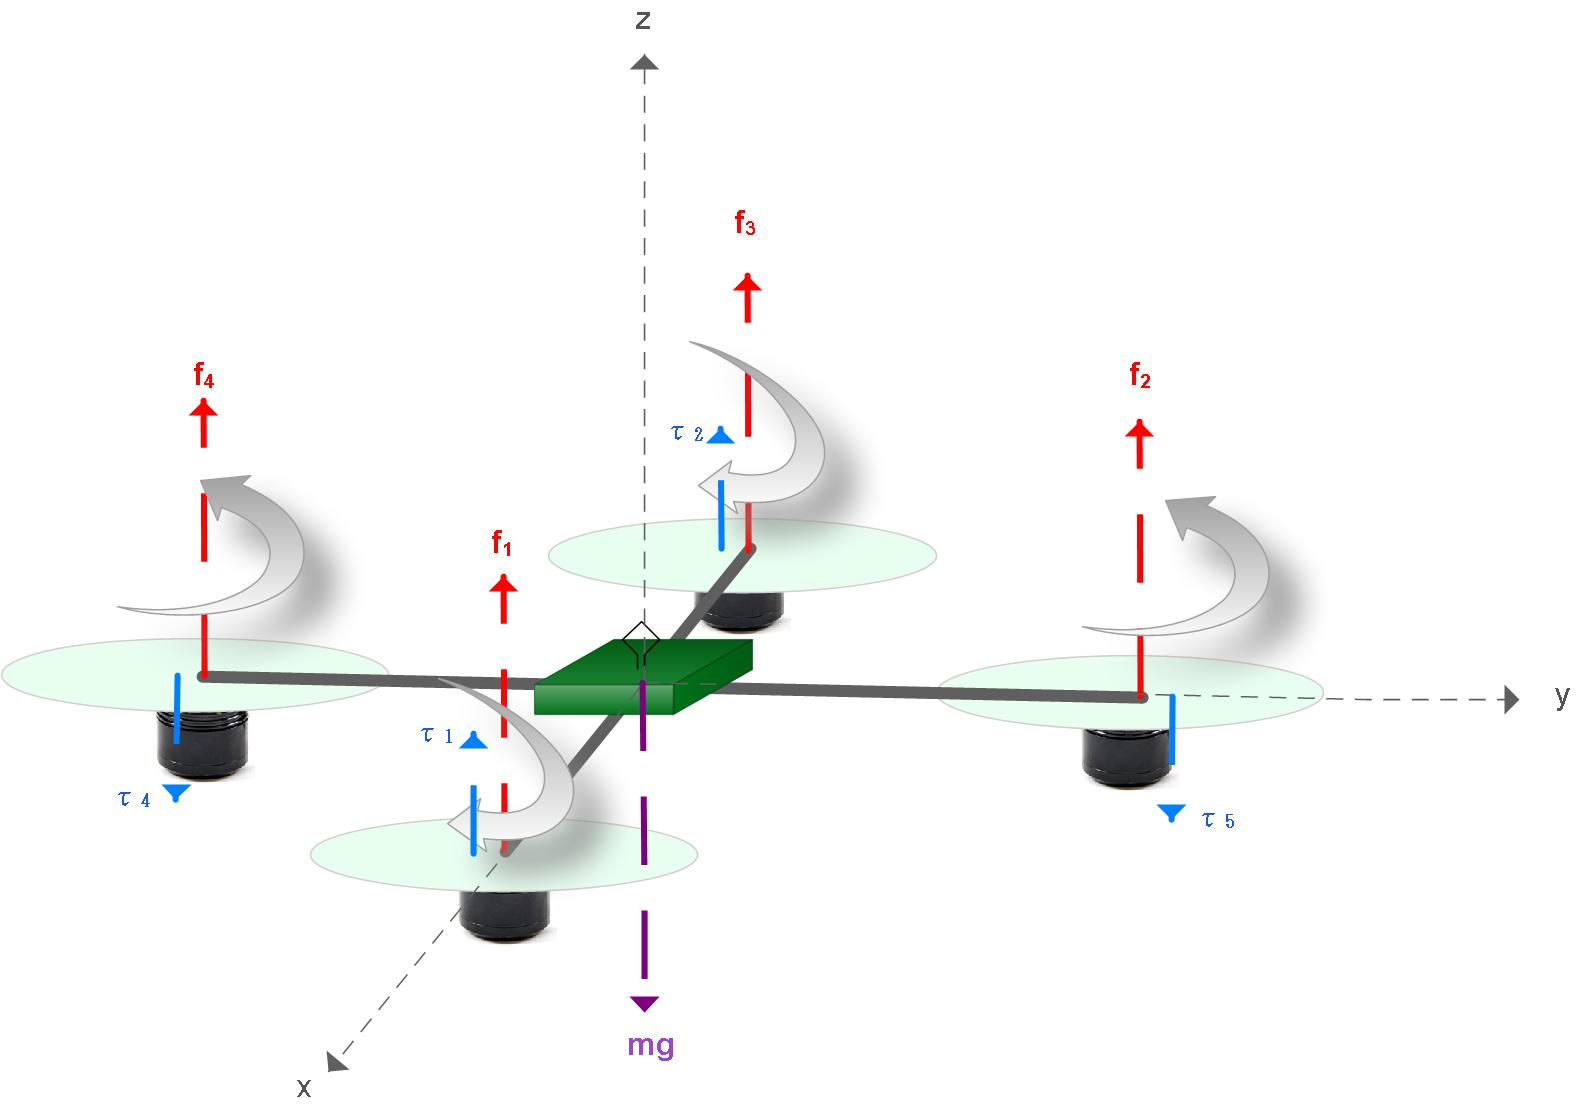
\includegraphics[scale=0.20]{Drone_diagram}
\end{center}
The model of position of a quadrotor can be written as:
\[ m\frac{d^{2}}{dt^{2}}\left( r \right)= F+F_{g} \]
Where 
\[ F= \sum_{i=1}^{4} f_{i}=\left( \begin{array}{c}
0\\0\\\sum_{i=1}^{4} f_{i}
\end{array} \right) \qquad F_{g}=\left(\begin{array}{c}
0\\0\\-mg
\end{array}\right) \]
$F$ is called the \emph{thrust} of the quadrotor. $f_{i}$ is the lift generated by each helix. This equation written in the inertial frame yields:
\[ m\frac{d^{2}}{dt^{2}}\left( \underset{\scriptscriptstyle S}{r} \right)= RF+F_{g} \]
$R$ is the rotation matrix and defines the body frame at time $t$. By developping this equation, it results:
\[ m\frac{d^{2}}{dt^{2}}\left( \begin{array}{c}
x\\y\\z
\end{array} \right) = \left( \begin{array}{c}
\ s\theta s\psi+c\theta s\phi c\psi\\-c\theta s\psi+s\theta s\phi c\psi\\c\phi c\psi
\end{array}\right) \left( \textstyle{\sum_{i=1}^{4} f_{i}} \right)+\left(\begin{array}{c}
0\\0\\-mg
\end{array}\right)
\]
\subsection{Attitude model of a quadrotor}
Concerning the part of rotation, the nex equation describes the behavior of a symmetric quadrotor:
\[ \frac{d}{dt}\left( Jw\right)=\tau \]
Where $J$ is the inertia matrix relative to body frame. $\tau$ represents the torques applied to quarotor.$J$ and $\tau$ have the following expressions: 
\[J=\left( \begin{array}{ccc}
J_{xx} & 0 & 0\\0 & J_{yy} & 0\\0 & 0 & J_{zz}
\end{array} \right) \qquad  \tau= \left( \begin{array}{c}
(f_{2}-f_{4})l\\(f_{3}-f_{1})l\\\sum_{i=1}^{4}\tau_{i}
\end{array} \right)=\left( \begin{array}{c}\tau_{xx} \\ \tau_{yy} \\ \tau_{zz}\end{array} \right)\]
$\tau_{i}$ is the drag torque generated by  the drag force on each helix. Now, writting the model in the inertial frame, it yields:
\[ \frac{d}{dt}\left( \underset{\scriptscriptstyle S}{Jw}\right)=\underset{\scriptscriptstyle S}{\tau} \]
\[ \frac{d}{dt}\left( RJw \right)=R \tau \]
\[ \dot{R}Jw+RJ\frac{dw}{dt}=R\tau \]
\[ RWJw+RJ\frac{dw}{dt}=R\tau\]
Therefore,
\[ J\frac{dw}{dt}=\tau-WJw\]
$W$ is the skew symmetric matrix defined before. Suppose it is true the following relationships:
\[ f_{i}=k_{f}{\Omega_{i}}^{2} \qquad \tau_{i}=(-1)^{i}k_{\tau} {\Omega_{i}}^{2}\quad \rm{for} \quad i \in [1,4] \]
$\Omega_{i}$ represents the rotation velocity of each helix. Thus, it can be written:
\[ \left( \begin{array}{c}
\tau_{xx}\\ \tau_{yy} \\ \tau{zz} \\ \sum_{i=1}^{4} f_{i}
\end{array} \right)=\left( \begin{array}{cccc}
0 & k_{f}l & 0 & -k_{f}l \\
-k_{f}l & 0 & k_{f}l & 0\\
k_{\tau} & -k_{\tau} & k_{\tau} & -k_{\tau}\\
k_{f}&k_{f} &k_{f} &k_{f}  
\end{array} \right) = \left( \begin{array}{c}
{\Omega_{1}}^{2}\\ {\Omega_{2}}^{2} \\ {\Omega_{3}}^{2} \\ {\Omega_{4}}^{2}
\end{array} \right) \]
This last equation is used to find the angular velocities of helices needed for generating specific torques anf thrust.\\[0.5cm]
Finally, the complete model is:
\[ \begin{array}{rcl}
{\displaystyle m\frac{d^{2}}{dt^{2}}\left( \underset{\scriptscriptstyle S}{r} \right) } & = & RF+F_{g}\\
{\displaystyle \frac{d}{dt}\left( R \right) }& = & RW\\
{\displaystyle J\frac{dw}{dt} } & = &\tau-WJw\\
\end{array} \]
\newpage
\section{Observations and conclusions}
The obtained model was developped assuming a rigid and symmetric quadrotor. In adittion, it is supposed  that gravity center is the same geometric center of the quadrotor. This can serve as a base for designing regulators and for observing their robustness even if the quadrotor has flexible structure and the gravity center is not accurate enough. A flexible structure can also originate a variation in the inertia tensor
\\[0.5cm]
Besides, it is considered that lift and drag forces can be calculated as a proprotion of square of angular velocities of each helix. This fact is not true if the quadrotor is near a wall or floor because the proportion can change. This model can be used as an approximation to behavior of the quadrotor.
\\[0.5cm]
Below some simulations regarding the behavior of quadrotor when applied specific forces and torques.
\begin{figure}[!h]
\begin{center}
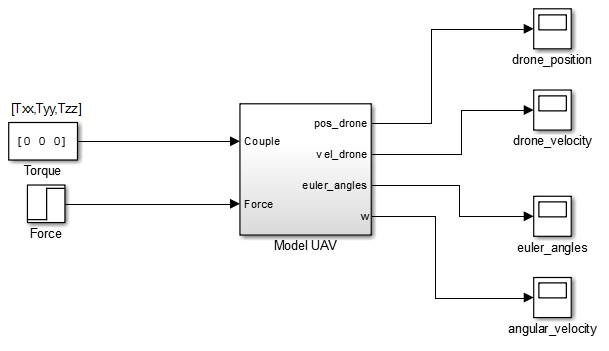
\includegraphics[scale=0.40]{Model_sml}
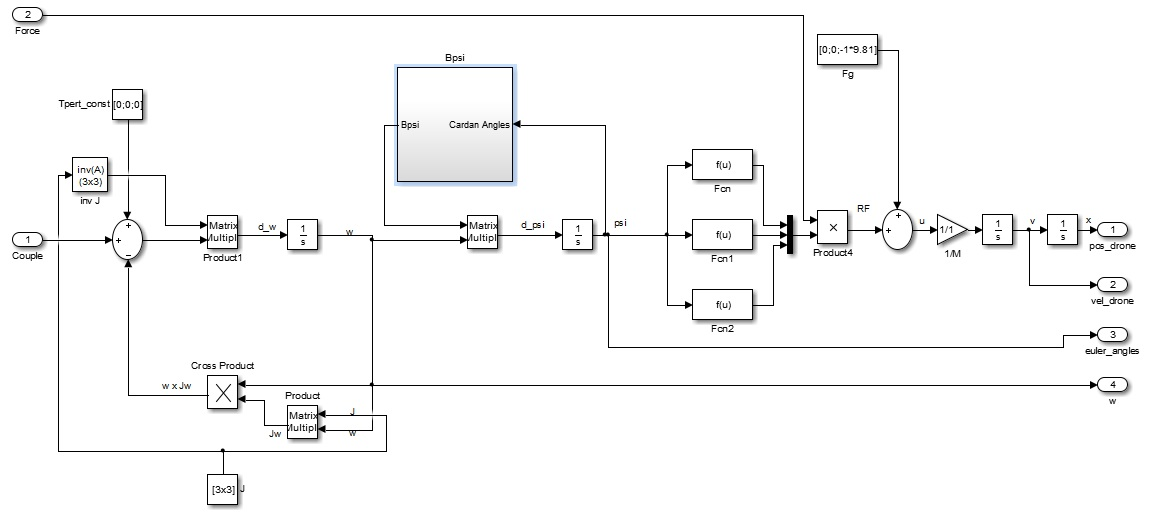
\includegraphics[scale=0.38]{Model_sml2}
\end{center}
\caption{Model of the quadrotor in simulink}
\end{figure}
The constants of the quadrotor during the simulation are:
\[ \mathbb{J}=diag(1,1,1) \quad m=1 \quad g=9.81 \quad Simulation time=10s\]
The first simulation is realized with constant thrust and nul torque. The second simulation is realized with constant thrust and constant torque in $x$ and nul torque in $y$ and $z$.The third simulation is realized with constant thrust and constant torque in $y$ and nul torque in $x$ and $z$.

\begin{figure}[H]
\begin{center}
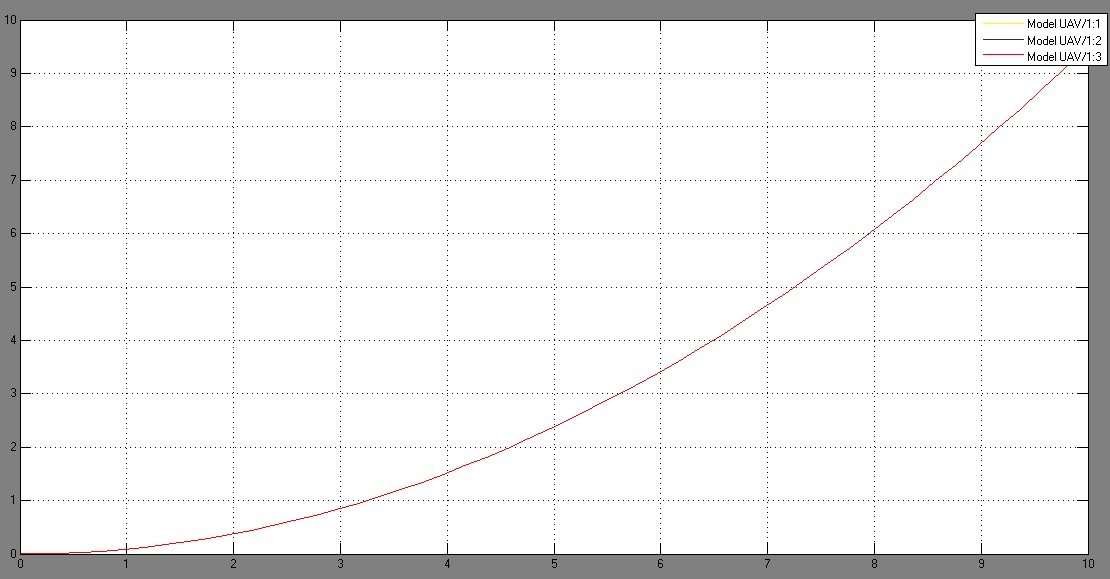
\includegraphics[scale=0.38]{Const_thrust}
\end{center}
\caption{Behavior with constant thrust and nul torque. Position-x=yellow line, position- y=blue line and position-z=red line}
\end{figure}

\begin{figure}[H]
\begin{center}
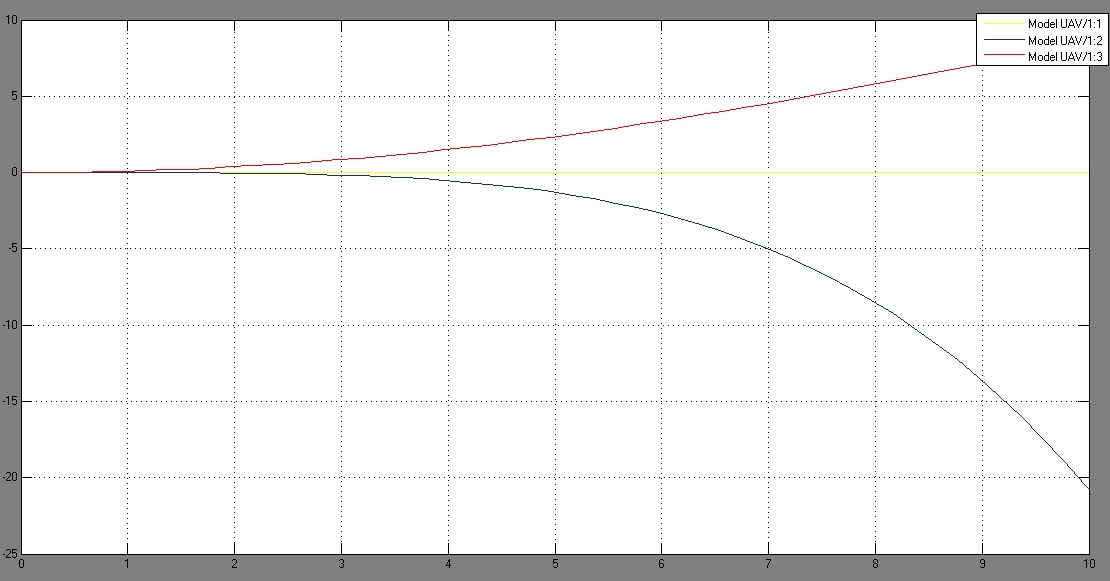
\includegraphics[scale=0.38]{Const_thrust_torque_x}
\end{center}
\caption{Behavior with constant thrust and constant torque in x. Position-x=yellow line, position- y=blue line and position-z=red line}
\end{figure}

\begin{figure}[H]
\begin{center}
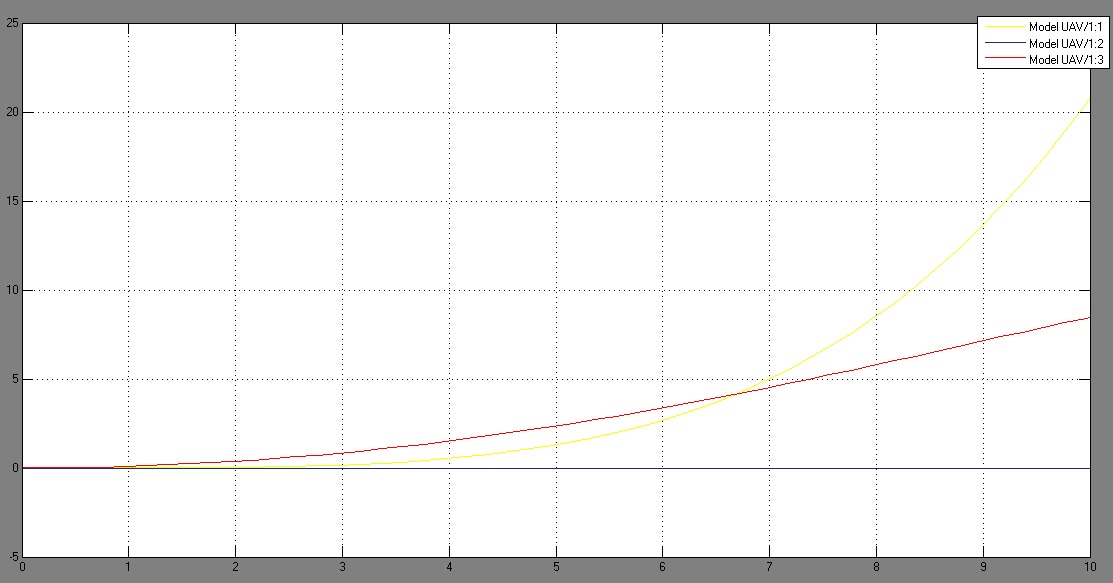
\includegraphics[scale=0.38]{Const_thrust_torque_y}
\end{center}
\caption{Behavior with constant thrust and constant torque in y. Position-x=yellow line, position- y=blue line and position-z=red line}
\end{figure}
\clearpage \newpage

\addcontentsline{toc}{section}{4. References}
\begin{thebibliography}{10}

\bibitem{Castillo}
  Pedro Castillo et al.,
  \emph{Modelling and Control of Mini-Flying Machines}.
  Springer Verlag,2005.  
  Chapter 3.
  
\bibitem{Naidoo}
  Yogianandh Naidoo et al.,
  \emph{QuadRotor Unmanned Aerial Vehicle Helicopter Modelling and Control }.
  2011.

\bibitem{Magnussen}
  �yvind Magnussen.
  \emph{Modeling, Design and Experimental Study for a Quadcopter System Construction}.
  MS Thesis 2011, Chapter 3.
  University of Agder.

\bibitem{Elruby}
  A. Y. Elruby et al.
  \emph{Dynamic Modeling and control of Quadrotor vehicle}.
  
\bibitem{Pounds}
  Paul Pounds et al.
  \emph{Modelling and Control of a Quad-Rotor Robot}.
  Australian National University.

\bibitem{Beard}   
   Beard and McLain .
   \emph{Small Unmanned Aircraft}.
   Princeton University Press, 2012.
   Chapter 3.
   
\bibitem{Barton}   
   Jeffrey D. Barton.
   \emph{Fundamentals of Small Unmanned Aircraft Flight}.
   Johns Hopkins APL Technical Digest.
   Volume 31, Number 2(2012).
   
   

\end{thebibliography}
\end{document}
